\chapter{Przegląd dostępnych rozwiązań}
\label{cha:przegladRozwiazan}

%---------------------------------------------------------------------------

\section{Najpopularniejsze standardy IdM}
\label{sec:standardyIdM}

Implementacja systemów zarządzania tożsamościami jest obszarem, w którym standaryzacja procesów wykorzystywania danych osobowych przynosi istotne korzyści. Wprowadzenie standardowych rozwiązań upraszcza wdrożenie nowych aplikacji lub usług typu "Identity Provider". Ujednoliceniu sposobu korzystania z funkcjonalności systemów zarządzania tożsamościami umożliwia tworzenie aplikacji klienckich używających podobnych rozwiązań dla dostępu do różnych usług. Rozwijanych jest wiele standardów realizujących wymagania stawiane systemom zarządzania tożsamościami. Najbardziej istotne z nich to SAML(Security Assertion Markup Language) oraz OpenID. 

\subsection{Security Assertion Markup Language}

	SAML to oparty na języku XML standard zarządzania tożsamościami oraz wymiany informacji uwierzytelniających \cite{Wisniewski05}. SAML oparty jest na podejściu wykorzystującym federację tożsamości - umożliwia tworzenie powiązań pomiędzy różnymi cyfrowymi tożsamościami użytkownika. SAML pozwala tworzyć asercje opisujące atrybuty tożsamości jednostki oraz przekazywać je do usług wymagających informacji identyfikujących swoich klientów.

	\subsubsection{Cele technologii SAML}

		Cele stawiane technologii SAML to\cite{Wisniewski05}:

		\begin{itemize}
		  \item niezależność od platformy - mechanizmy bezpieczeństwa powinny być niezależne od środowiska i implementacji usługi.
		  \item luźne powiązanie pomiędzy elementami wchodzącymi w skład infrastruktury opartej o wymianę komunikatów SAML
		  \item uproszczenie procesu uwierzytelniania z perspektywy klienta, np. poprzez wprowadzenie procedury SSO
		  \item redukcja kosztów administracyjnych poprzez zastąpienie wielu oddzielnych modułów bezpieczeństwa jednym wspólnym dla  różnych aplikacji
		\end{itemize}

	\subsubsection{Struktura specyfikacji SAML}

		Specyfikacja technologii SAML definiuje czterowarstwową strukturę, w skład której wchodzą asercje, protokoły, mapowania dla protokołów komunikacyjnych oraz profile. 
		Asercje zawierają informacje wymieniane pomiędzy aplikacjami, usługami "Identity Provider" oraz użytkownikami. Protokoły, mapowania oraz profile definiują mechanizmy przetwarzania asercji.

		\paragraph{Asercje}\mbox{}\\
					
			Asercje są to wiadomości zawierające dane identyfikacyjne jednostek w systemie. Składają się z deklaracji tożsamości opisujących jednostki wygenerowanych przez usługę "Identity Provider" systemu SAML. Na podstawie otrzymanych deklaracji tożsamości jednostki dostawca usługi podejmuje decyzję o przyznaniu lub odmówieniu prawa dostępu do swoich zasobów. Również dostawcy usług mają możliwość tworzenia asercji w celu utworzenia zapytania do serwisu uwierzytelniającego o parametry transakcji określania tożsamości. 

			\subparagraph{Struktura asercji}\mbox{}\\
			
				\begin{figure}[h]
				\centering
					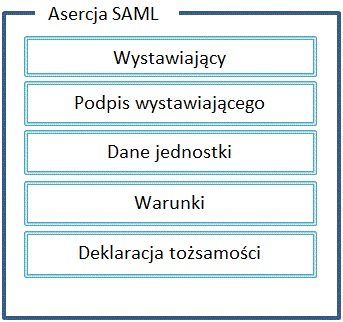
\includegraphics{img/samlAssertion.jpg}
				\caption{Elementy asercji SAML}
				\label{Elementy asercji SAML}
				\end{figure}

				Asercja SAML zawiera informacje o wystawiającym asercję. Może zawierać również informację o dacie wygenerowania asercji. W celu zapewnienia integralności informacji do asercji dołączany jest cyfrowy podpis wystawiającego. W dalszej części asercji znajdują się dane opisujące jednostkę, względem której utworzono asercję. Następną sekcją wiadomości są warunki, pod którymi asercja może być wykorzystywana. W tym fragmencie mogą znajdować się informacje o okresie ważności asercji lub usługi, do których adresowana jest asercja. Ostatnim elementem jest deklaracja tożsamości, zawierające informacje kontekstowe o procesie uwierzytelniania, np. dotyczące zastosowanej metody uwierzytelniania.

			\subparagraph{Typy deklaracji tożsamości}\mbox{}\\

				Specyfikacja definuje następujące typy deklaracji tożsamości zawartych w asercjach SAML\cite{Wisniewski05}:

				\begin{itemize}
				  \item deklaracja uwierzytelniania - stwierdza, że opisana w asercji jednostka została uwierzytelniona w danym momencie przy użyciu mechanizmów opisanych w opisie kontekstu deklaracja
				  \item deklaracja atrybutu - stwierdza, że dany atrybut o zadanej wartości jest przypisany jednostce
				  \item deklaracja autoryzacji - stwierdza, że jednostce opisanej w asercji przyznano lub odmówiono praw dostępu do zasobów pod określonymi warunkami
				 \end{itemize}

		\paragraph{Protokoły}\mbox{}\\ 

			Protokoły SAML definiują format wiadomości żądań i odpowiedzi pozwalających na komunikację pomiędzy elementami systemu zarządzania tożsamościami przy pomocy technologii SAML. Specyfikacja SAML określa protokoły:

			\begin{itemize}
			  \item protokół odpytywania usługi "Identity Provider" o asercje
			  \item protokół żądania uwierzytelniania jednostki
			  \item protokół rejestrowania identyfikatorów jednostek
			  \item protokół żądania wygaśnięcia identyfikatora jednostki
			  \item protokół żądania jednokrotnego wylogowania z wielu aplikacji
			  \item protokół żądania odzwierciedlenia pomiędzy różnymi identyfikatorami jednostki
			\end{itemize}

		\paragraph{Mapowania dla protokołów komunikacyjnych}\mbox{}\\

			Mapowania SAML do protokołów komunikacyjnych określają w jaki sposób wiadomości protokołów SAML powinny być przekazywane przy pomocy standardowych protokołów komunikacyjnych.  Mapowania mogą np. definiować sposób przesyłania wiadomości SAML przy pomocy protokołów HTTP lub SOAP.

		\paragraph{Profile}\mbox{}\\

			Profile SAML definiują zbiór funkcjonalności jakie można uzyskać przy użyciu elementów niższych warstw(asercji, protokołów i mapowań) oraz sposób w jaki te funkcjonalności mogą być osiągnięte. Przykładem mogą być profile jednokrotnego uwierzytelniania specyfikujące sposób komunikacji pomiędzy dostawcami usług i serwisami "Identity Provider" w celu dostarczenia mechanizmów SSO lub profile zapytania o asercję dla jednostki.

	\subsubsection{Mechanizmy jednokrotnego uwierzytelniania przy użyciu SAML}

		\paragraph{Schemat funkcjonowania mechanizmów SSO w oparciu o technologię SAML}\mbox{}\\

			\begin{figure}[h]
				\centering
					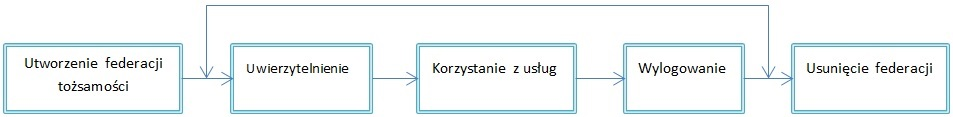
\includegraphics[width=15cm,height=2.5cm]{img/samlSSO.jpg}
				\caption{Schemat funkcjonowania mechanizmu jednokrotnego uwierzytelniania w SAML}
				\label{Schemat funkcjonowania mechanizmu jednokrotnego uwierzytelniania w SAML}
			\end{figure}

			Aby istniała możliwość korzystania z mechanizmu jednokrotnego uwierzytelniania konieczne jest utworzenie federacji pomiędzy tożsamościami jednostki. Po utworzeniu powiązań pomiędzy różnymi tożsamościami użytkownik po poprawnym uwierzytelnieniu względem jednej z usług może korzystać z innych sfederowanych serwisów. Wylogowanie się wykonane dla którejś z aplikacji powoduje zamknięcie dostępu do wszystkich sfederowanych usług. Procedura jednokrotnego uwierzytelniania może być wykorzystywana do momentu usunięcia federacji pomiędzy tożsamościami użytkownika.

		\paragraph{Przebieg procesu jednokrotnego uwierzytelniania w SAML}\mbox{}\\

			\begin{figure}[h]
				\centering
					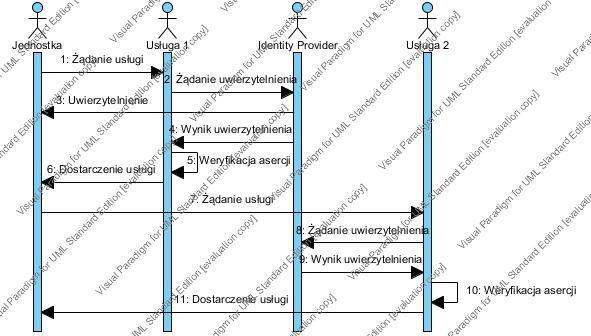
\includegraphics[width=15cm,height=10cm]{img/ssoSteps.jpg}
				\caption{Przebieg procesu jednokrotnego uwierzytelniania w SAML}
				\label{Przebieg procesu jednokrotnego uwierzytelniania w SAML}
			\end{figure}

			Usługa objęta mechanizmem jednokrotnego uwierzytelniania po otrzymaniu żądania udostępnienia swoich zasobów zleca modułowi "Identity Provider" przeprowadzenie procesu uwierzytelnienia klienta serwisu. Asercja będąca wynikiem procesu uwierzytelnienia zostaje przekazana do usługi zlecającej. Usługa dokonuje weryfikacji otrzymanej asercji i akceptuje lub odrzuca żądanie dostępu do zasobów. Gdy użytkownik chce skorzystać z usług innego serwisu sfederowanego z usługą, do której otrzymał dostęp, proces uwierzytelniania przebiega podobnie. Pomijany jest jednak krok ponownego uwierzytelniania użytkownika przez usługę "Identity Provider" - usługa ta zwraca do aplikacji żądającej uwierzytelniania asercję wygenerowaną na podstawie wcześniej wykonanego procesu uwierzytelniania.	
			
\subsection{OpenID}

OpenID

\subsection{Liberty Identity Web Services Framework}

	Identity Web Services Framework(ID-WSF) to zbiór specyfikacji definiujących mechanizmy dla zapewnienia bezpieczeństwa serwisów webowych, pomiędzy którymi istnieją relacje zaufania(federacje)\cite{Oracle10}. ID-WSF określa podejście do zarządzania tożsamościami, w którym tożsamości jednostek zarządzane są przez różnych dostawców usług połączonych relacją federacji. Usługi webowe mogą wymieniać między sobą dane osobowe swoich użytkowników w celu dostarczenia funkcjonalności żądanej przez klienta usługi. Przykładem sytuacji, gdzie może być zastosowany ten model jest usługa potrzebująca dostarczenia danych adresowych swojego użytkownika. W tym celu może skorzystać z zasobów innej usługi 
	dysponującej tymi danymi.

	Rysunek przedstawia przebieg procesu współdzielenia informacji w ID-WSF. Specyfikacja ID-WSF wprowadza dodatkowy element do architektury systemów zarządzania tożsamościami - "Discovery Service". Usługa "Discovery Service" pozwala dostawcom usług na wyszukiwanie innych serwisów dostarczających funkcjonalności pozwalających na realizacje żądań zadanych usłudze. Klient aplikacji decyduje o tym czy jego dane mogą być dostępne dla innych serwisów rejestrując usługę dostarczającą jego danych osobowych w rejestrze "Discovery Service" lub nie dokonując takiej rejestracji. Na przedstawionym schemacie żądana przez użytkownika usługa potrzebuje dodatkowych informacji - w tym celu w rejestrze usług szuka serwisu, który dostarcza potrzebnych informacji dla obsługiwanego użytkownika.

	\begin{figure}[h]
		\centering
			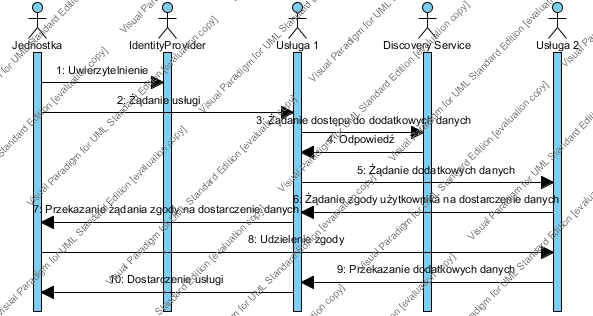
\includegraphics[width=15cm,height=9cm]{img/id-wsf.jpg}
		\caption{Przebieg procesu wykorzystywania informacji dzielonych w ID-WSF}
		\label{Przebieg procesu wykorzystywania informacji dzielonych w ID-WSF}
	\end{figure}

	ID-WSF definiuje również mechanizmy pozwalające na komunikację pomiędzy dostawcami usług i użytkownikiem w celu uzyskania zgody na przekazanie danych osobowych do innej aplikacji. Zaprezentowany diagram przedstawia ten proces. Usługa 2. po otrzymaniu żądania dostarczenia dodatkowych danych os Usługi 1. wymaga zgody użytkownika na udzielenie wymaganych informacji.
	
%---------------------------------------------------------------------------

\section{Przykłady frameworków zarządzających uwierzytelnianiem i autoryzacją użytkowników}
\label{sec:frameworki}
	\subsection{Protokół Kerberos}

		Kerberos jest protokołem uwierzytelniania użytkowników zasobów sieciowych.

		\subsubsection{Cele protokołu Kerberos}

			Centralnym punktem architektury Kerberos jest serwer uwierzytelniający. Każda komponent systemu Kerberos jest połączony z serwerem uwierzytelniającym relacją zaufania; wszystkie żądania uwierzytelniania są kierowane do tego serwera. Działanie systemu Kerberos opiera się na usługach KDC(Key Distribution Center). Każdy serwis KDC posiada bazę użytkowników i usług wraz z ich danymi uwierzytelniającymi. Dzięki temu możliwe jest uproszczenie zadań administracyjnych. Pozwala to również zastosować bardziej skuteczne mechanizmy bezpieczeństwa chroniące bazę użytkowników.

			Kerberos zapewnia bezpieczeństwo procesu uwierzytelniania gwarantując przesyłanie danych uwierzytelniających w postaci zaszyfrowanej. Korzysta z biletów(ang. Tickets) - wiadomości kryptograficznych dowodzących tożsamości użytkownika żądającego dostępu do zasobów serwera. Bilety dostarczane są przez usługę KDC na żądanie uwierzytelniającego się klienta. Bilety wystawiane są najczęściej na pewien okres - po jego upływie tracą ważność. Bazując na generowanych biletach Kerberos dostarcza mechanizmu jednokrotnego uwierzytelniania. 

			Zastosowanie protokołu Kerberos gwarantuje obustronne uwierzytelnienie w procesie komunikacji pomiędzy klientem a serwerem - zarówno klient jak i serwer muszą dowieść swojej tożsamości. 

		\subsubsection{Elementy systemu Kerberos}

			Każdy użytkownik, usługa lub host w systemie Kerberos ma przypisany unikalny w ramach domeny identyfikator. Każdy identyfikator skojarzony jest z kluczem uwierzytelniającym jednostkę w systemie. Kluczem tym może być np. hasło. Identyfikatory wraz z kluczami przechowywane są w bazie usługi "Key Distribution Center". W skład KDC wchodzi również serwer uwierzytelniający i serwer TGS(Ticket Granting Server). W systemie Kerberos może istnieć więcej niż jedna usługa KDC - istnieje konieczność synchronizacji zawartości bazy identyfikatorów dla każdej z usług KDC.

			Serwer uwierzytelniający przyznaje zaszyfrowany bilet - Ticket Granting Ticket(TGT) - użytkownikowi uwierzytelniającemu się w domenie. Użytkownik nie musi przesyłać usłudze swoich danych uwierzytelniających ponieważ zwracany bilet TGT jest szyfrowany hasłem użytkownika. Otrzymany bilet może być wykorzystany aby otrzymać bilet specyficzna dla zasobów, do których użytkownik chce uzyskać dostęp. Bilety specyficzne dla określonej usługi przyznawane są przez serwer TGS. Serwer dokonuje weryfikacji otrzymanych biletów TGT, sprawdzając czy jest on poprawnie zaszyfrowany kluczem serwera Kerberos. Po zakończonej powodzeniem weryfikacji serwer przyznaje bilet specyficzny dla żądanej usługi.

	\subsection{Standard WS-Security}

		WS-Security to standard specyfikujący rozszerzenia protokołu SOAP(Simple Object Access Protocol) pozwalające na zagwarantowanie mechanizmów uwierzytelniania, poufności komunikacji oraz integralności dostarczania danych dla usług sieciowych opartych o technologię SOAP. Standard ten oparty jest na koncepcji zapewnienia mechanizmów bezpieczeństwa na poziomie przesyłanych wiadomości\cite{Hallam03}. 

		Specyfikacja WS-Security umożliwia uwierzytelnianie użytkownika usługi poprzez definicję formatu przesyłania tokenów bezpieczeństwa. Token bezpieczeństwa pozwala na dostarczenie danych uwierzytelniających użytkownika(np. identyfikatora i hasło) lub asercji opisującej tożsamości klienta usługi. Tokeny bezpieczeństwa mogą być szyfrowane, możliwe jest również zastosowanie certyfikatów X.509 potwierdzających tożsamość jednostki dostarczającej token. 

		Standard WS-Security pozwala na zapewnienie poufności komunikacji poprzez zastosowanie szyfrowania wiadomości SOAP. Szyfrowana może być cała wiadomość lub tylko jej części. WS-Security definiuje również mechanizmy gwarantowania integralności dostarczanych komunikatów. Do tego celu wykorzystywane są podpisy XML. 

	\subsection{Standard WS-Trust}

		Standard WS-Trust rozszerza specyfikację WS-Security definiując metody wystawiania, odnawiania i weryfikacji tokenów bezpieczeństwa oraz sposoby ustanawiania relacji zaufania pomiędzy dostawcami usług i klientami. Podobnie jak specyfikacja WS-Security, standard WS-Trust nie jest zależny od konkretnego protokołu bezpieczeństwa - umożliwia zastosowanie różnych protokołów\cite{WS-Trust-1.4-with-errata}.

		W modelu definiowanym przez standard WS-Trust usługa oczekuje dołączenia do wiadomości informacji potwierdzających tożsamość klienta. Serwis powinien odrzucać żądania bez dołączonych wymaganych informacji. Wymagane przez serwis dane mogą być wskazane w opisie polityki usługi. Polityki mogą być definiowane przy użyciu standardu WS-Policy. Uwierzytelnianie nadawcy wiadomości może być oparte o mechanizmy bezpieczeństwa warstwy transportowej, dane dostarczone w żądaniu SOAP lub poprzez szyfrowanie wiadomości kluczem znanym nadawcy. Jednym ze sposobów gwarancji korzystania z autoryzowanego tokenu bezpieczeństwa jest dołączenie do informacji cyfrowego podpisu szyfrowanego poufnym kluczem skojarzonym z tokenem.

		Standard WS-Trust wprowadza pojęcie usługi "Security Token Service"(STS). Jest to usługa przyznająca klientom tokeny bezpieczeństwa, które później mogą być wykorzystane w celu uwierzytelnienia i autoryzacji dostępu do innych usług. W celu dostarczenia tokenu STS wymaga najczęściej danych uwierzytelniających klienta(np. identyfikatora i hasła). Tokeny przyznawane przez usługę STS umożliwiają nawiązywanie relacji zaufania pomiędzy różnymi domenami bezpieczeństwa. Specyfikacja określa również sekwencje wymieniany komunikatów dla różnych scenariuszy pozyskiwania tokenu bezpieczeństwa. Zastosowanie usługi "Security Token Serie" umożliwia uwierzytelnianie, kontrolę dostępu do zasobów, nadzór nad działaniem systemu bezpieczeństwa oraz nawiązywanie relacji zaufania.

		\begin{figure}[h]
			\centering
				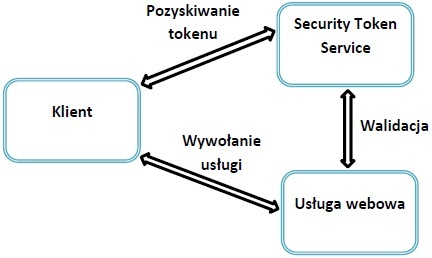
\includegraphics{img/ws-trust.jpg}
			\caption{Model zapewnienia bezpieczeństwa dostępu do aplikacji w standardzie WS-Trust}
			\label{Model zapewnienia bezpieczeństwa dostępu do aplikacji w standardzie WS-Trust}
		\end{figure}

		Klient może pozyskiwać tokeny bezpieczeństwa od usługi "Security Token Serie". Otrzymany token może być dołączony do żądania klienta wysyłanego do usługi webowej. Serwis powinien weryfikować czy usługa wystawiająca token objęta jest relacją zaufania względem danych, które dostarcza. Serwis może ufać otrzymywanym tokenom bezpieczeństwa lub zlecać i walidację usłudze STS. Usługa może również komunikować się z modułem STS w celu wymiany otrzymanego tokenu bezpieczeństwa na inny odpowiedni dla mechanizmów bezpieczeństwa danej usługi. 

		Serwis może deklarować kryteria dla otrzymywanych tokenów określające kiedy token będzie uznany za zaufany\cite{WS-Trust-1.4-with-errata}. Możliwe kryteria to np.:

		\begin{itemize}
			\item typ tokenu(np. token protokołu Kerberos)
			\item dostawca tokenu - usługa deklaruje dostawców tokenów, dla których istnieje relacja zaufania
			\item hierarchia zaufania - usługa może określać zaufanie względem jednostek, w których hierarchii zaufania znajduje się określony serwis
			\item zaufanie tylko dla tokenów wystawianych przez serwis uwierzytelniający - otrzymane tokeny przekazywane są do usługi uwierzytelniającej; w procesie udostępniania zasobów wykorzystywany jest token wygenerowany przez tą usługę na podstawie tokenu dostarczonego w żądaniu. 
		\end{itemize} 
		
	Informowanie odbiorców usług o wymaganiach bezpieczeństwa stawianych przez serwis jest możliwe dzięki standardowi WS-SecurityPolicy. Jest to specyfikacja rozszerzająca język WSDL(Web Services Description Language) pozwalająca definiować następujące wymagania bezpieczeństwa:

	\begin{itemize}
		\item konieczność dostarczenia tokenu bezpieczeństwa
		\item konieczność dostarczenia podpisu dla tokenu bezpieczeństwa
		\item wymagany sposób szyfrowania
		\item konieczność dostarczenia cyfrowego podpisu dla określonej części wiadomości
		\item konieczność szyfrowania określonej części wiadomości
		\item wymaganie dostarczenia określonych wiadomości opisujących klienta aplikacji
	\end{itemize} 

	\subsection{Standard WS-Federation}

		Standard WS-Federation definiuje mechanizmy pozwalające na dzielenie tożsamości i atrybutów jednostek pomiędzy usługami w różnych domenach administracyjnych lub domenach bezpieczeństwa w oparciu o reguły i wymagania zdefiniowane przy pomocy mechanizmu polityk\cite{Goodner09}. Specyfikacja określa sposób współdzielenia informacji dotyczących bezpieczeństwa pomiędzy usługami dostarczającymi tokenów bezpieczeństwa a dostawcami usług. Definicja polityk umożliwia deklarację danych, które mogą być współdzielone. Wymieniane informacje mogą obejmować dane o sfederowanych usługach, wymagania zawarte w politykach federacji, opis relacji zaufania oraz tokeny bezpieczeństwa.

		Koncepcja federacji w standardzie WS-Federation wprowadza mechanizm mapowania tożsamości. Jest to proces translacji cyfrowej tożsamości pomiędzy formatem rozumianym przez domenę nadawcy a formatem akceptowanym przez domenę docelową. Usługa dokonująca mapowania tożsamości powinna posiadać relację zaufania dla domeny nadawcy i mieć uprawnienia do przekazywania informacji do domeny odbiorcy.

		Specyfikacja WS-Federation wykorzystuje model pozyskiwania tokenów bezpieczeństwa i uwierzytelniania przy ich pomocy opisywany w standardzie WS-Trust. Standard WS-Federation rozszerza koncepcję opisaną w WS-Trust o możliwość pozyskiwania informacji o politykach realizowanych przez usługi i stawianych przez nie wymaganiach dotyczących zabezpieczania dostępu do chronionych zasobów. Specyfikacja określa sposób wykorzystania modeli opisanych przez WS-Security, WS-Trust i WS-Policy tworząc bardziej rozbudowany model relacji zaufania pomiędzy serwisami przy użyciu mechanizmu federacji.

		\begin{figure}[h]
			\centering
				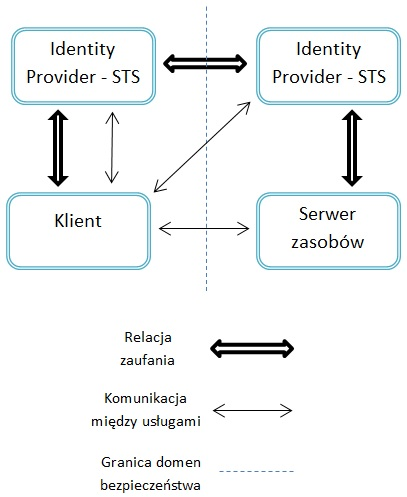
\includegraphics{img/ws-federation.jpg}
			\caption{Prosty scenariusz federacji serwisow}
			\label{Prosty scenariusz federacji serwisow}
		\end{figure}

		Przedstawiony schemat ilustruje przebieg uzyskiwania dostępu do zasobu przy użyciu mechanizmu federacji. Przerywana linia stanowi granicę między domenami bezpieczeństwa. Klient przeprowadza proces uwierzytelniania  i uzyskuje token bezpieczeństwa od usługi "Security Token Service" w swojej domenie bezpieczeństwa. Otrzymany token zostaje przedstawiony usłudze STS w odrębnej domenie bezpieczeństwa w celu uzyskania tokenu uprawniającego do dostępu do zasobów w tej domenie. Token uzyskany w tym procesie jest przesyłany w żądaniach dostępu do zasobów w odrębnej domenie bezpieczeństwa. 

	\subsection{Standard OAuth}

		W podstawowej koncepcji ograniczania dostępu do zasobów użytkownik uzyskuje dostęp do zasobów korzystając z dany uwierzytelniających właściciela zasobu. Gdy klient usługi chce udostępnić usłudze chronione zasoby musi przekazać jej swoje dane uwierzytelniające.  Zastosowanie tego modelu pociąga za sobą zagrożenia bezpieczeństwa związane z przechowywaniem dany uwierzytelniających przez usługę, której udzielono dostępu do danych, brakiem możliwości ograniczenia udzielonych praw dostępu jedynie do części zasobów oraz brakiem możliwości odebrania przydzielonych wcześniej praw dostępu.

		Jednym z rozwiązań tego typu problemów jest zastosowanie standardu OAuth - specyfikacji definiującej mechanizmy autoryzacji dostępu do zasobów dla protokołu HTTP\cite{Hardt12}. Standard OAuth zakłada wprowadzenie dodatkowej warstwy autoryzacji  oraz rozdzielenie ról klienta i właściciela zasobu. W procesie przyznawania klientowi praw dostępu do zasobu wykorzystywane są dane uwierzytelniające różne od danych właściciela zasobu. W tym celu klient otrzymuje token dostępu od serwera autoryzującego za zgodą właściciela zasobu. Token zawiera m. in. informacje określające zakres praw nadanych użytkownikowi oraz okres obowiązywania przyznanych uprawnień. 

		Właścicielem zasobów w standardzie OAuth jest jednostka przyznająca dostęp do zasobów. Klientem jest aplikacja, która w odpowiedzi na operacje wykonywane przez  właściciela zasobu i za jego zgodą korzysta z tego zasobu.

		\begin{figure}[h]
			\centering
				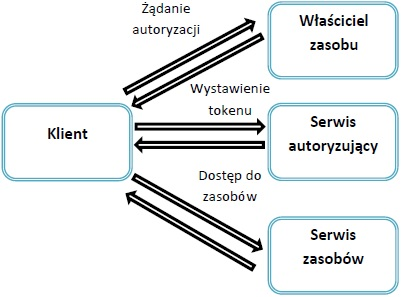
\includegraphics{img/oauth.jpg}
			\caption{Przebieg autoryzacji w standardzie OAuth}
			\label{Przebieg autoryzacji w standardzie OAuth}
		\end{figure}

		Proces przyznania klientowi dostępu do zasobu rozpoczyna się żądaniem autoryzacji przesyłanym do właściciela zasobu.  Właściciel zasobu odpowiada na żądanie przesyłając grant autoryzujący typu zależnego od metody wykorzystywanej do autoryzacji. Następnie klient przysyła do serwera autoryzującego żądanie przydzielenia tokenu dostępu na podstawie otrzymanego grantu autoryzującego. Serwer autoryzujący uwierzytelnia klienta i weryfikuje otrzymany grant autoryzujący i na tej podstawie przyznaje token dostępu. Klient korzysta z zasobów przedstawiając przydzielony mu token dostępu.

%---------------------------------------------------------------------------

